% vim: set tw=78 sts=2 sw=2 ts=8 aw et ai:
\documentclass[12pt]{article}

\usepackage[paper=a4paper, top=2cm, bottom=3cm, left=2.5cm, right=2.5cm]{geometry}

\usepackage{ucs}
\usepackage[utf8x]{inputenc}
\usepackage[english]{babel}
%\usepackage{hyperref}	  % use \url{http://$URL} or \href{http://$URL}{Name}
\usepackage{underscore}	  % underscores need not be escaped
\usepackage{subfigure}
\usepackage{verbatim}
\usepackage{float}
\usepackage{booktabs}     % professional tables
\usepackage{parskip}

% hyper-references
% http://www.tug.org/applications/hyperref/manual.html
\usepackage{hyperref}
\hypersetup{%
	colorlinks=true,
	linkcolor=blue,
	anchorcolor=black,
	citecolor=black,
	filecolor=blue,
	menucolor=black,
	urlcolor=blue,
	bookmarks=true,
	bookmarksnumbered=true
}
\urlstyle{sf}

% command for specifying TODOs
\newcommand{\todo}[1]{
	\colorbox{yellow}{
		\begin{minipage}{15cm}
			\textbf{TODO:}\\
			#1
		\end{minipage}
	}
}

% Support for including graphics
\usepackage{graphicx}
\graphicspath{ {img/} }
\DeclareGraphicsExtensions{.pdf,.png,.jpg}

\title{Disaster Management}

\author{Ioana Ciornei, Vladimir Oltean\\
Faculty of Automatic Control and Computers\\
University POLITEHNICA of Bucharest\\
Splaiul Independenței 313, Bucharest, Romania, 060042 \\
\emph{\{ciorneiioana,olteanv\}@gmail.com}}

\date{\today}

\begin{document}

\maketitle

\begin{abstract}
% vim: set tw=78 sts=2 sw=2 ts=8 aw et ai:
In this paper we describe a prototype client-server application for disaster
management. Information about the location of all clients is gathered
centrally by the server, which is then able to take the best-informed decision
on behalf of them, by using Multiple Criteria Decision Analysis.

\end{abstract}

\section{Introduction}
\label{sec:introduction}
% vim: set tw=78 sts=2 sw=2 ts=8 aw et ai:

In the circumstances of a disaster (either natural or caused by man), there is
generally a high level of confusion among large groups of people. The
immediate action that needs to be taken is usually finding a safe spot to
hide. Afterwards, one can attempt to eliminate the cause of the disaster and
rescue the people left behind.

Because of the general confusion, the immediate decision to escape that is
made by the individual may be based only on intuition, and thus not optimal.

This project's goal is to create a mobile application that helps the user in an
emergency situation by pointing to the best safe place to hide. The list of
alternatives for shelter can either be crowdsourced from the other
participants to the disaster, or provided by the owner of the venue themselves
(say for example an accident happens during a concert or sports game).

The application has a component which is permanently running in the background
as a service, and keeps listening for events that might trigger an emergency
alert.

Once emergency state is triggered, the active part of the application, in the
form of an activity, is automatically brought to the user's foreground, and
guides them to the best known safe spot.

While being a scenario that lends itself well to a mesh network approach, the
proposed prototype follows a traditional approach with a single, centralized
server. This is responsible for receiving messages from all mobile clients,
either sharing their current location, or the location of a newfound shelter.

The server keeps track of the positions of all clients and safe spots. On
request, it will apply a decision-making algorithm and select the most
appropriate safe location for the client who is asking.

The client is able to customize the way safe locations are being selected by
the server. As part of the decision-making algorithm, the user's perceived
importance of the following criteria is taken into consideration:

\begin{itemize}
  \item Proximity to the respective exit point. If this is perceived as
    important to the user, the server will tend to prefer guiding this user
    towards exit points that are close to him, with a higher precedence over
    other criteria.
  \item Safety of the exit point. This can be rephrased as "guarantee that
    the user can indeed exit through that point". A simple way to measure this
    (negatively) is to count the number of people who are in the vicinity of
    that exit spot, but cannot pass through it.
  \item How crowded is the exit point. The metric proposed here is the speed
    that people in the exit's vicinity are able to pass through it. A
    congested exit point permits people to exit at a much lower rate than one
    that is free. The difference between the metric used for crowdedness and
    the one used for safety is the fact that crowdedness only looks at the
    people who managed to escape, while safety looks at those who didn't.
  \item Being close to friends.
\end{itemize}


\section{Architecture}
\label{sec:architecture}

\subsection{Server}
\label{sec:server}
% vim: set tw=78 sts=2 sw=2 ts=8 aw et ai:

The server is composed of multiple services that are all part of a process
running in a Java VM:

\begin{itemize}
  \item Android Proxy Service. This handles communication between the clients
        and the other services.
  \item Android Client Service. This keeps track of the trajectory and safety
        status of each mobile client over time.
  \item Safe Location Service. This is used to store information about exit
        points that is learned from the clients.
  \item Criteria Score Calculator and Spark Service. These are the modules
        involved in the computation of the optimal exit path requested by
        clients.
\end{itemize}

Communication with clients is done over TCP sockets, as JSON-formatted messages.
The following message types can be sent unidirectionally by the clients, and
no response is expected back from the server:

\begin{itemize}
  \item "client-location": A client can communicate its current position to
        the server, who will store it in the Android Client Service.
  \item "safe-location": Clients also have the ability to inform the server
        about exit points. In the current implementation this information is
        trusted blindly by the server, but future iterations should use
        techniques such as Bayesian inference to establish a degree of
        certainty about the actual safety of these locations. Note that
        upon receiving a new safe location, no action is taken by the server
        to inform the other connected clients about it, since this must be
        solicited explicitly.
  \item "friends": Clients can tell the server about other clients they wish
         to stay near to.
  \item "delete-clients" and "delete-safe-locations": These commands were used
        in the development phase of the application, in order to initiate the
        simulation of a new emergency event.
\end{itemize}

There is another category of client messages for which the server is expected
to send a response:

\begin{itemize}
  \item "safe-location-preferences": Should be sent at the beginning of the
        communication by the client, to inform the server of its preference
        for the 4 possible criteria: "safety", "proximity", "notCrowded" and
        "closeToFriends". A "consistency-ratio" response is expected from the
        server, informing the client whether the provided information make
        sense and can be used in the decision-making algorithm.
  \item "safe-location-request": This message triggers the decision making
        algorithm on the server, customized with the requesting client's
        information and preferences. A "safe-location-response" is issued on
        the way back, giving the latitude and longitude of the selected best
        exit point, along with its score in the decision algorithm.
\end{itemize}

The Multiple-Criteria Decision Analysis (MCDA) algorithm used is Analytic
Hierarchy Process (AHP) \cite{ahp}. The 4 criteria are structured on Level 1,
while the n Safe Location alternatives are positioned on Level 2 of the
hierarchy.

In the first stage of the algorithm, a priority vector (containing criteria
weights) is calculated based on the client's preferences received as input.

In the second stage, for all n alternative Safe Locations, 4 priority vectors
are calculated, one for each criterion (safety, proximity, crowdedness and
closeness to friends). These hold the actual scores of the Safe Locations
computed by the server from the perspective of that specific criterion.

The final priority vector is calculated by weighing the individual scores
obtained by the Safe Locations with the user's specific preferences with each
criterion.

For some criteria (for example crowdedness), computation is performed on the
Apache Spark cluster. The list of clients is converted to an RDD, and at the
end of the computation a score for the Crowded criterion is output.

\begin{figure}
\centering
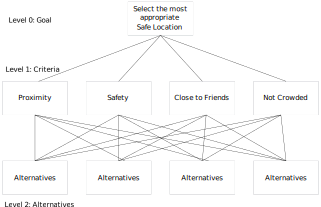
\includegraphics[scale=0.3]{ahp}
\caption{\label{fig:ahp} Analytic Hierarchy Process}
\end{figure}



\subsection{Client}
\label{sec:client}
The client side is implemented as an Android application, \textit{DMDataGenerator}, that gathers location data for its users, interracts with the server and, if needed, it communicates a possible \textit{safe location} to the user.

Taking into consideration the fact that we have developed this client application as an easy way of testing the underlying management algorithm, there are multiple ways of using it, as a user but also as a developer:

\begin{itemize}
\item Generate data samples
\item Combine data samples into custom new ones
\item Replay samples
\item Choose preferences in terms of what means a \textit{safe location}
\item Choose friends
\end{itemize}

In the next paragraphs we will briefly describe each structural component of the client application and also the protocol used to communicate with the server.

\begin{wrapfigure}{R}{0.3\textwidth}
\centering
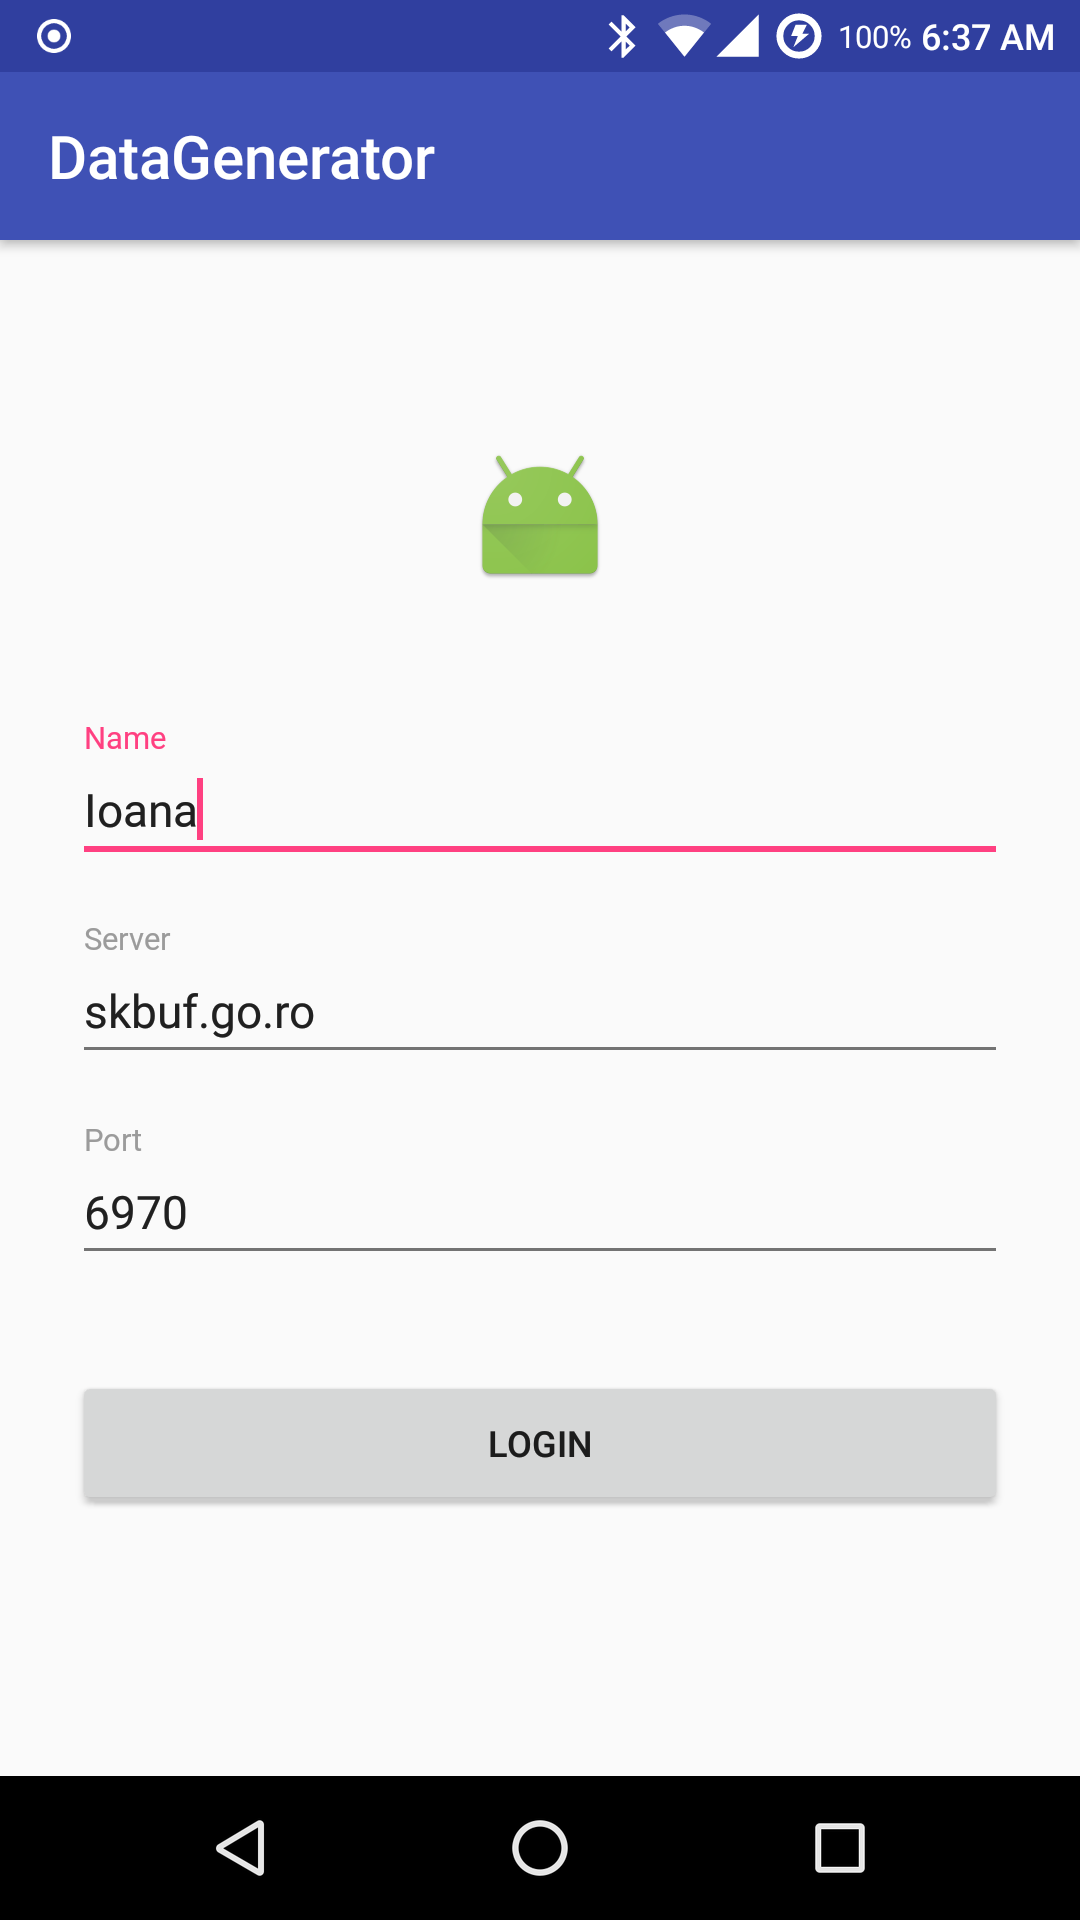
\includegraphics[scale=0.1]{login}
\caption{\label{fig:login}Login Activity}
\end{wrapfigure}

Using the \textit{Login Activity}, Figure \ref{fig:login}, an user can manually select the address of the server and also an username to be used throughout the application. 

\begin{wrapfigure}{R}{0.3\textwidth}
\centering
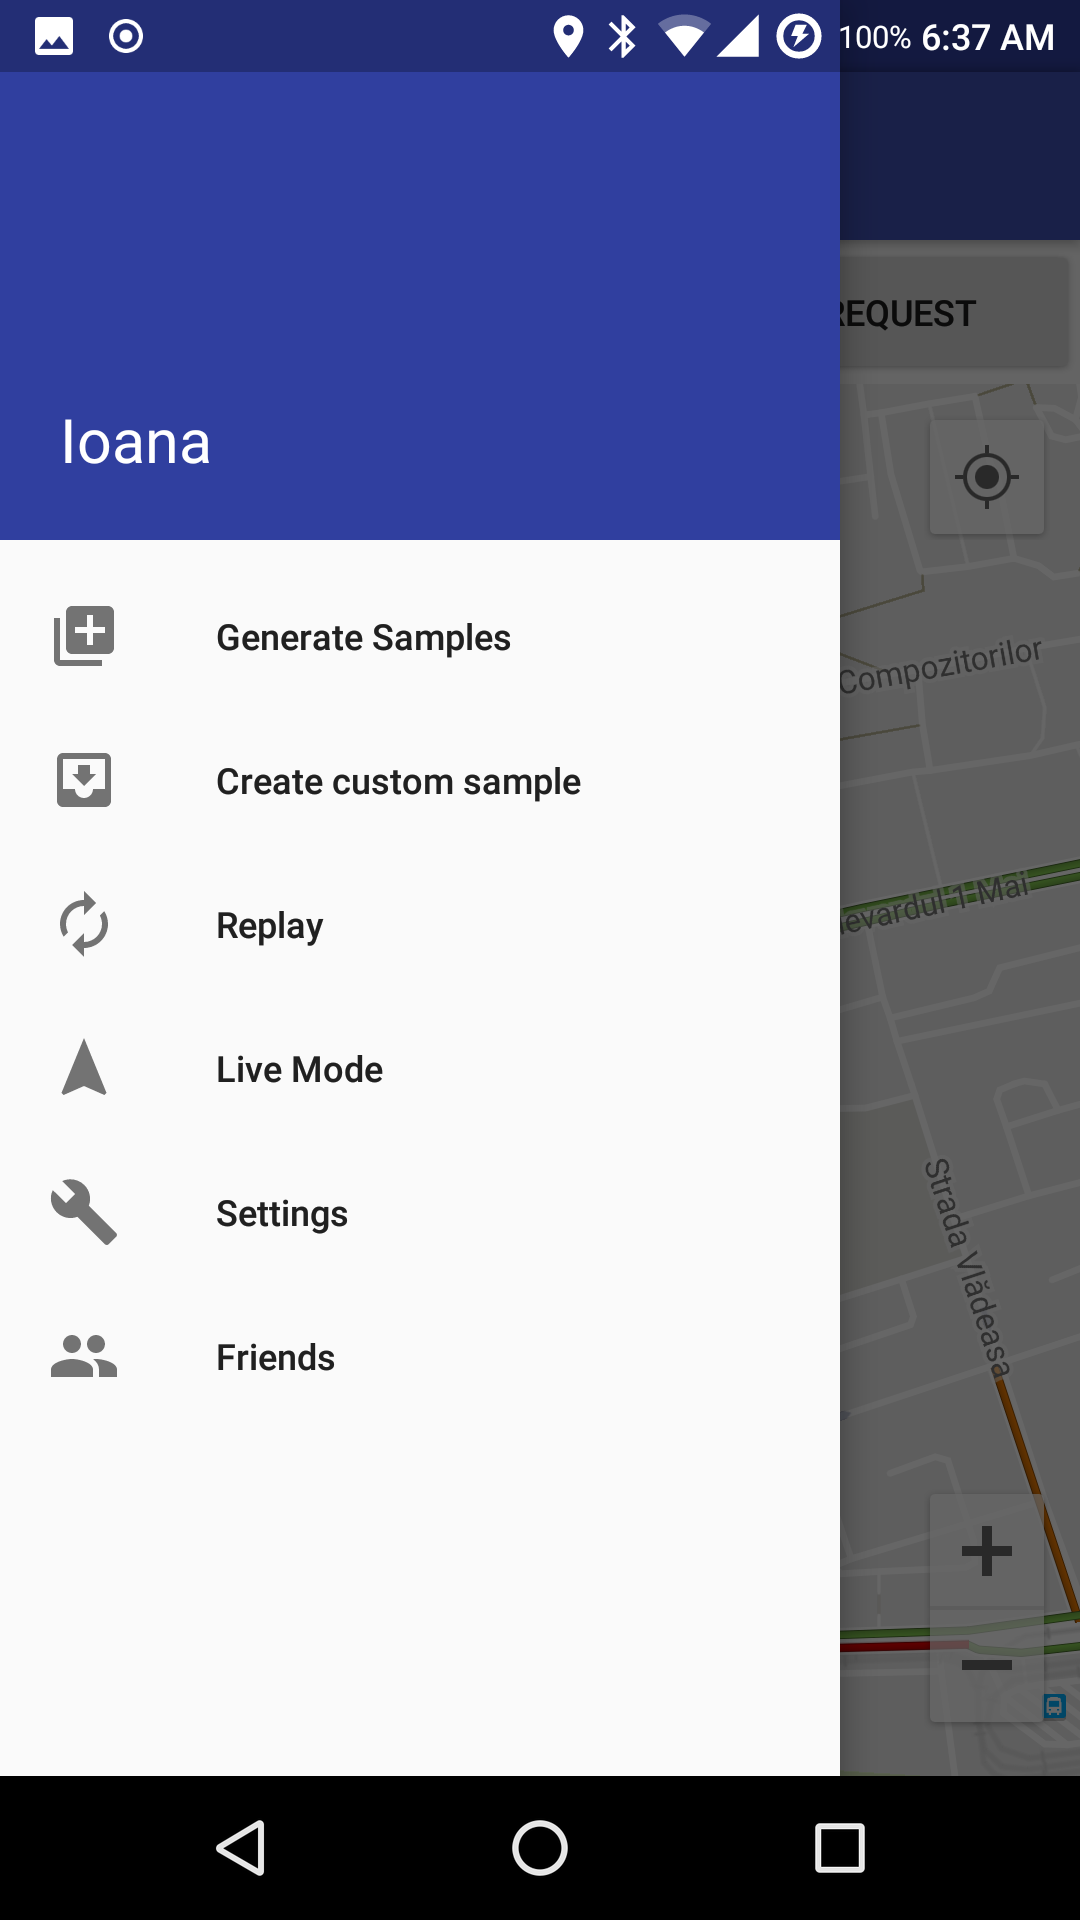
\includegraphics[scale=0.1]{menu}
\caption{\label{fig:menu} Menu sidebar}
\end{wrapfigure}

By pressing \textit{Login}, the user is redirected to the \textit{MainActivity}. There, using the options presented in the \textit{Menu Sidebar - Figure \ref{fig:menu}}, an user can easily navigate through features.

\begin{wrapfigure}{R}{0.3\textwidth}
\centering
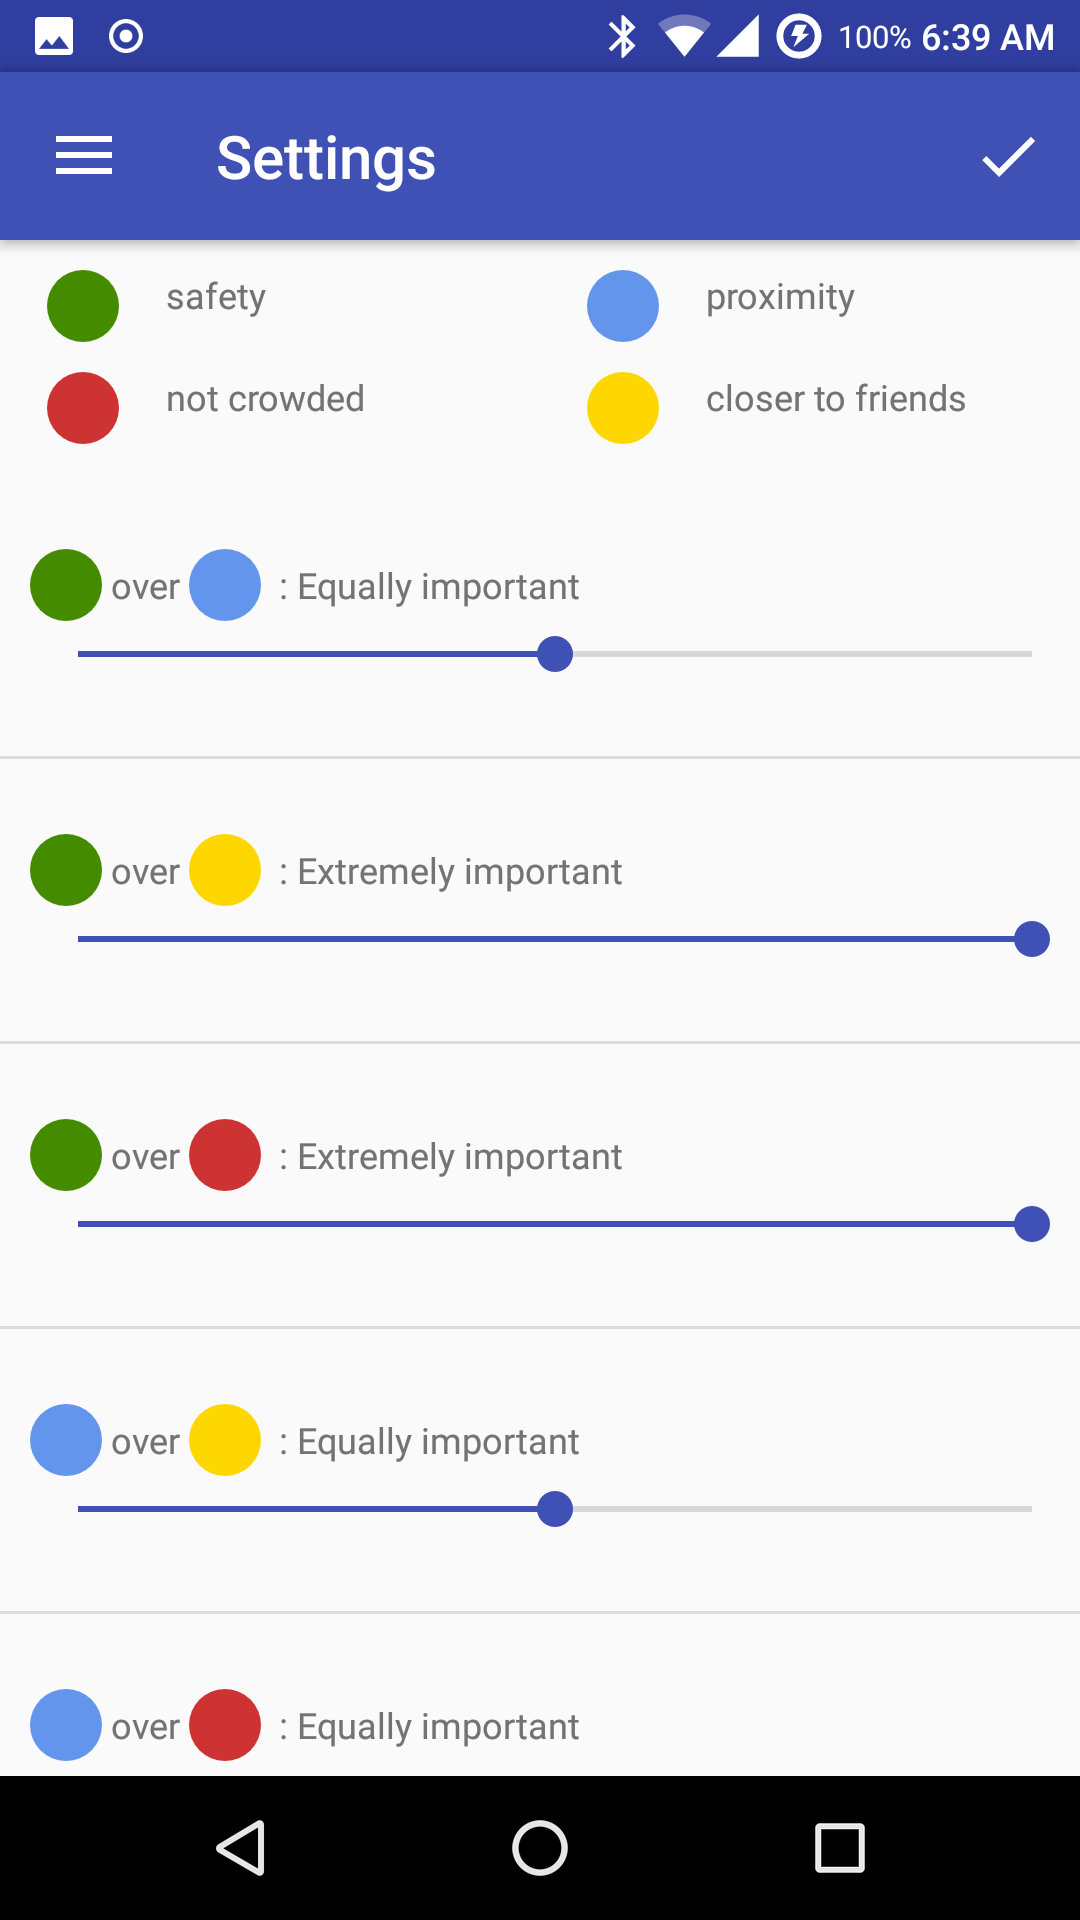
\includegraphics[scale=0.1]{settings}
\caption{\label{fig:settings}Settings Activity}
\end{wrapfigure}

Before trying to generate or manipulate data samples, an user must set its preferences using the menu item - \textit{Settings - Figure \ref{fig:settings}}.

As stated before in the Introduction - Chapter \ref{sec:introduction}, one can customize, depending on its preferences, the way a \textit{safe location} is defined.

Starting from the 4 criteria described above, one can specify the importance of one over another. And because consistency of preferences must be always met, an user can always verify if everything is in order using the check toolbar button.

\begin{wrapfigure}{R}{0.3\textwidth}
\centering
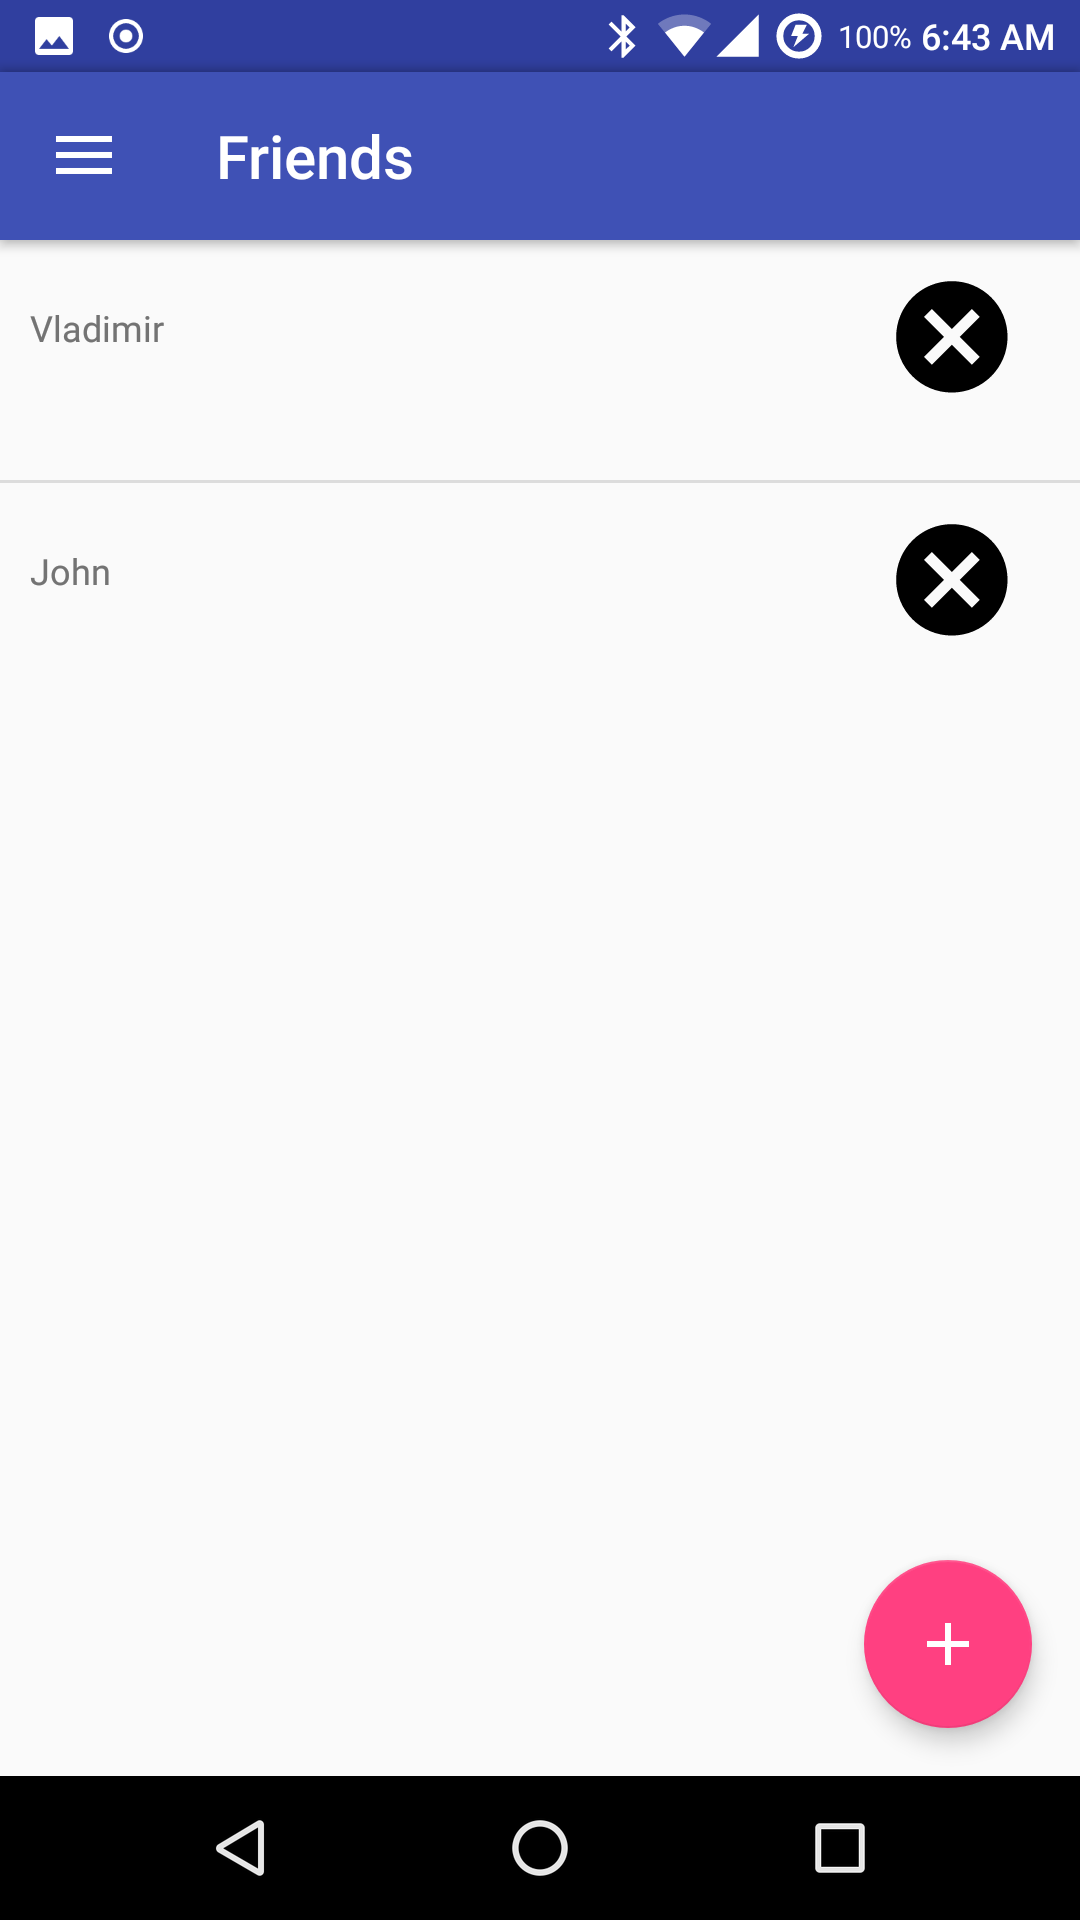
\includegraphics[scale=0.1]{friends}
\caption{\label{fig:friends}Friends Activity}
\end{wrapfigure}

\textit{Proximity to friends} is one of the criteria used to evaluate a possible \textit{safe spot} thus specifiying other users trated as friends is possible using the \textit{Friends Activity - Figure \ref{fig:friends}}.

When interracting with the server, user preferences and also friends names are transformed into JSON formatted messages, as explained above. In this specific case, message types \textit{safe-location-preferences} and \textit{friends} are used.

\begin{wrapfigure}{R}{0.3\textwidth}
\centering
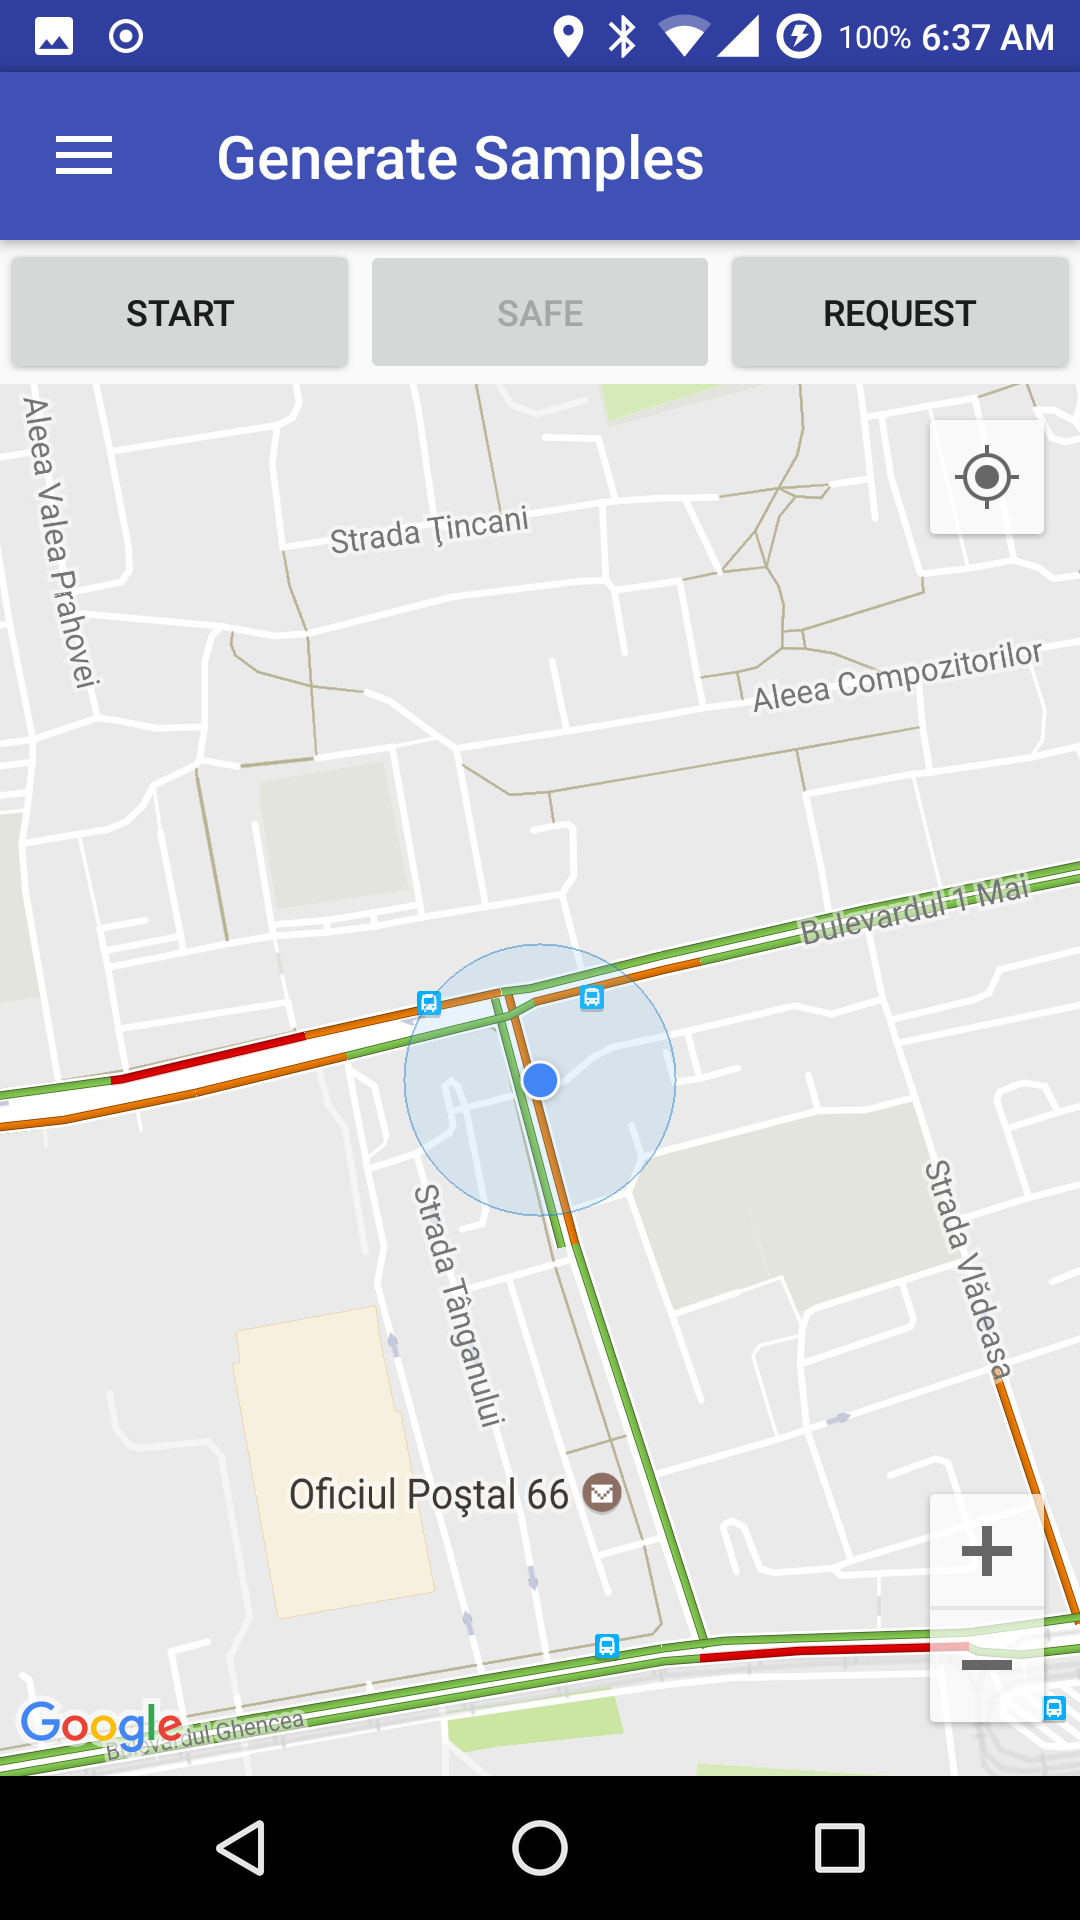
\includegraphics[scale=0.1]{generate}
\caption{\label{fig:generate}Generate Sample Activity}
\end{wrapfigure}

Using \textit{Generate Sample Activity - Figure \ref{fig:generate}}, one can create data samples based on location updates provided by GoogleAPIs. The user is given the option of announcing that he/she found a \textit{safe spot} or to request one from its peers. Upon termination, a text file with the \textit{sample-timestamp-username} format is created on the external storage (/sdcard/DMDataGenerator-Samples).

\lstset{
    string=[s]{"}{"},
    stringstyle=\color{blue},
    comment=[l]{:},
    commentstyle=\color{black},
}

%\begin{lstlisting}
%{"msgtype":"delete-clients"}
%{"msgtype":"delete-safe-locations"}
%{"msgtype":"friends","name":"111","friends":["22"]}
%{"msgtype":"safe-location-preferences","name":"111","criteria":["safety","proximity","closeToFriends","notCrowded"],"pairwiseComparisons":[4.0,4.0,4.0,1.0,1.0,1.0]}
%{"msgtype":"client-location","name":"111","timestamp":998,"latitude":44.418954,"longitude":26.0436168}
%{"msgtype":"client-location","name":"111","timestamp":1998,"latitude":44.4189502,"longitude":26.0436203}
%{"msgtype":"safe-location-request","timestamp":43752,"name":"111"}
%{"msgtype":"safe-location","name":"111","timestamp":7389,"latitude":44.4188103,"longitude":26.0443281}
%\end{lstlisting}


\begin{wrapfigure}{R}{0.3\textwidth}
\centering
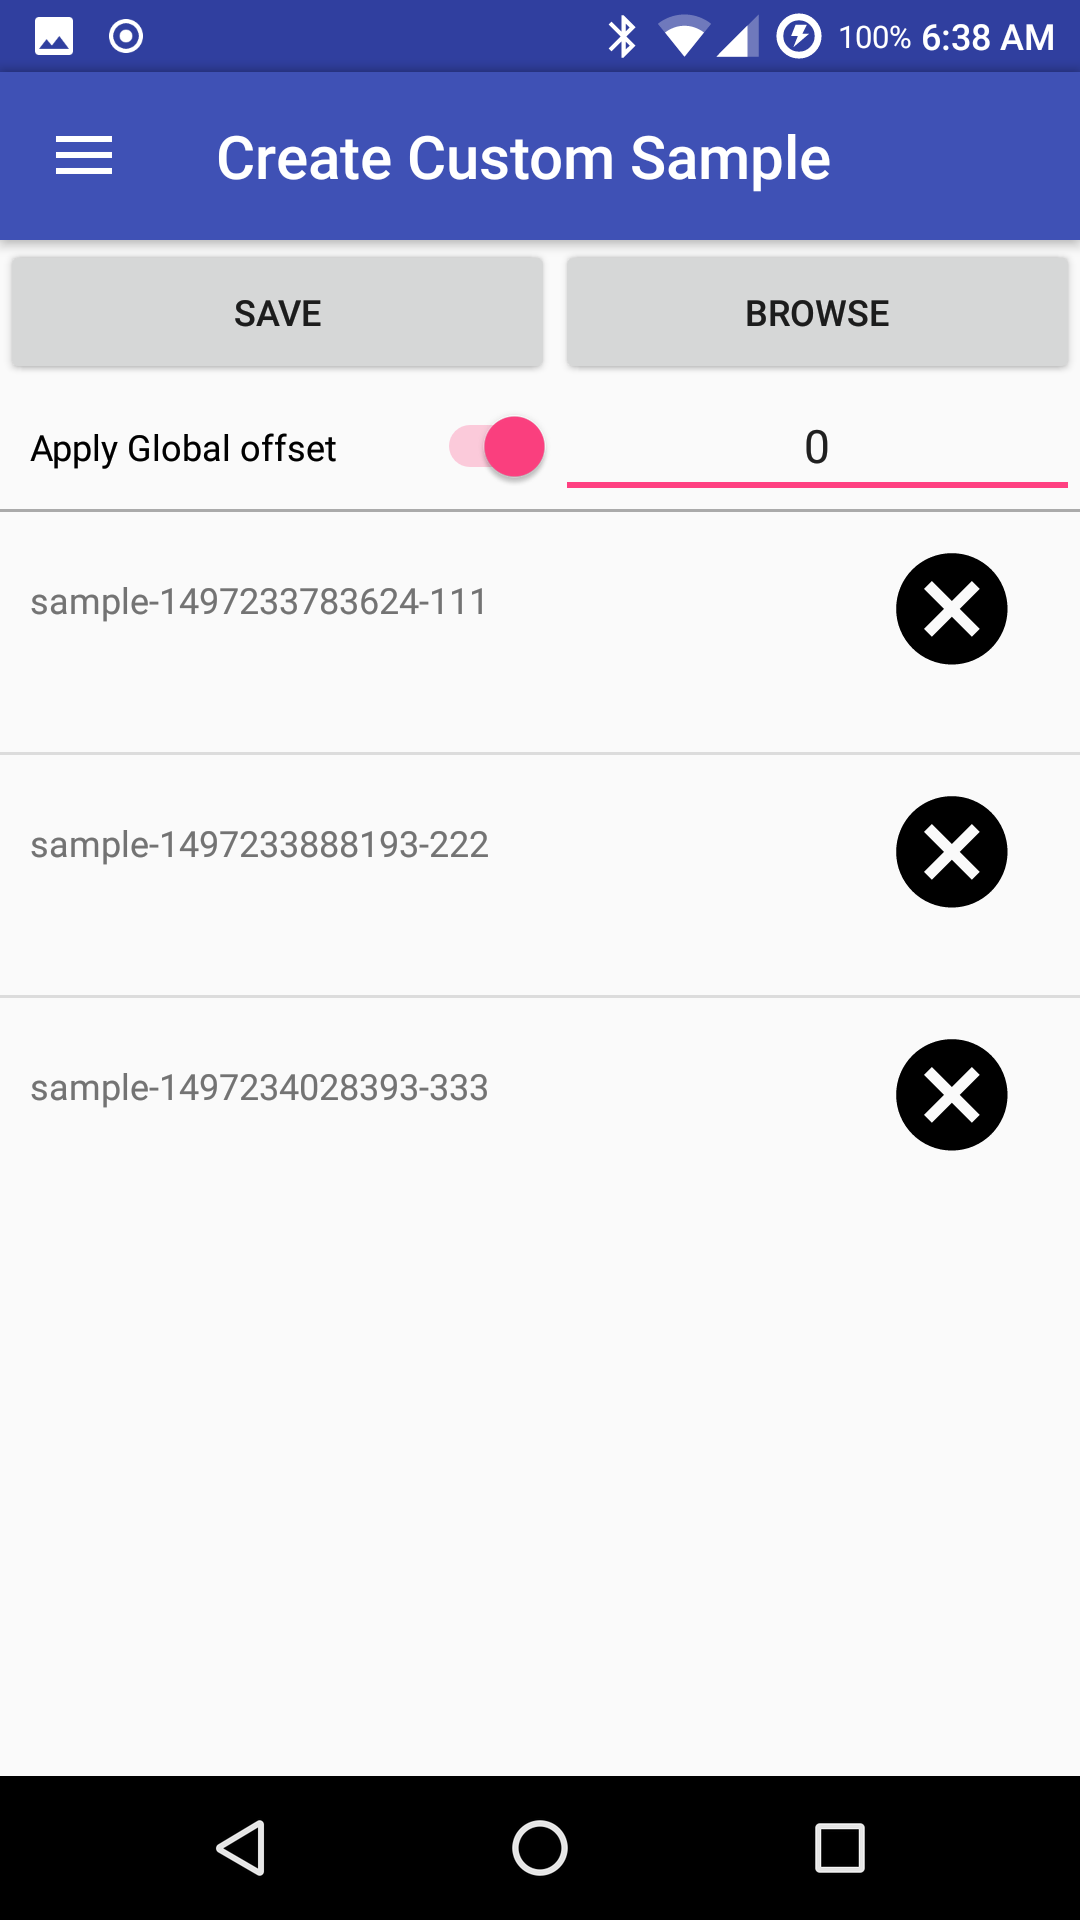
\includegraphics[scale=0.1]{custom}
\caption{\label{fig:custom}Create Custom Sample Activity}
\end{wrapfigure}

\begin{wrapfigure}{R}{0.3\textwidth}
\centering
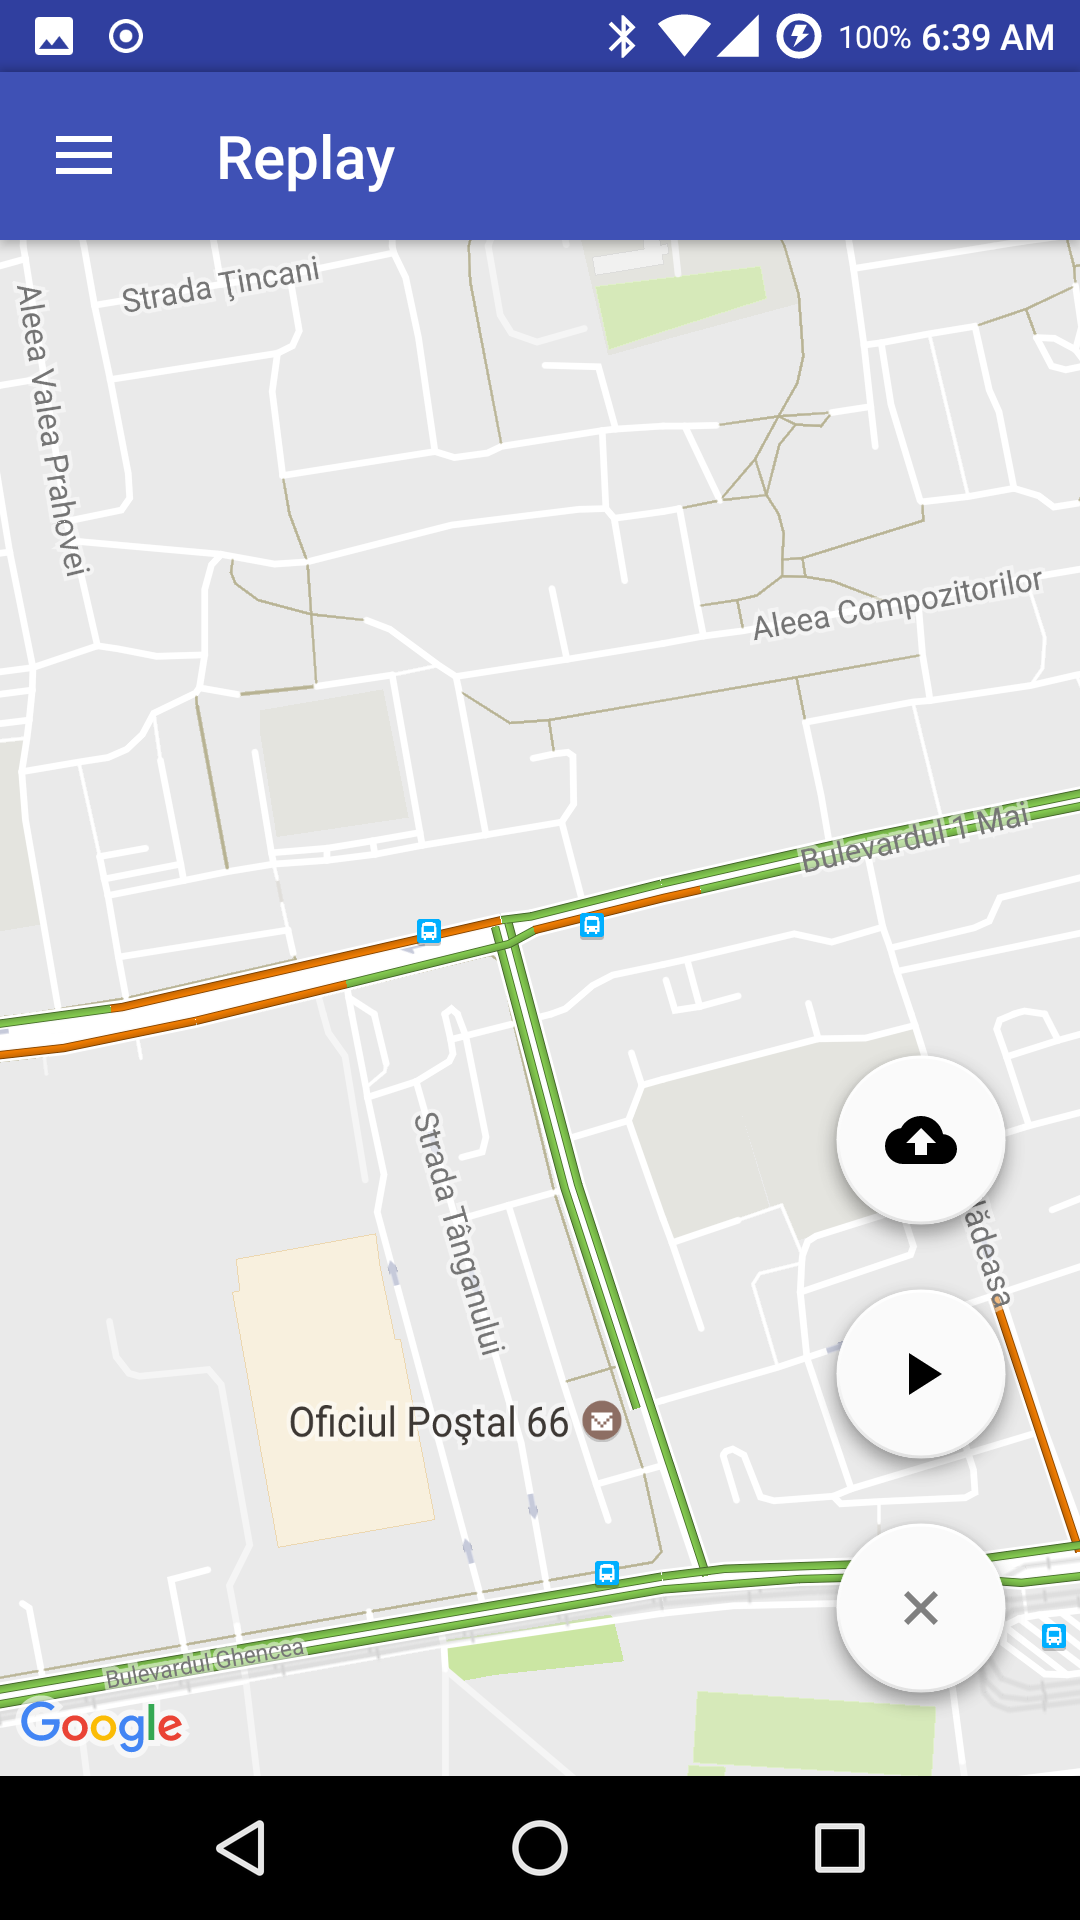
\includegraphics[scale=0.1]{replay}
\caption{\label{fig:replay}Replay Activity}
\end{wrapfigure}

\begin{wrapfigure}{R}{0.3\textwidth}
\centering
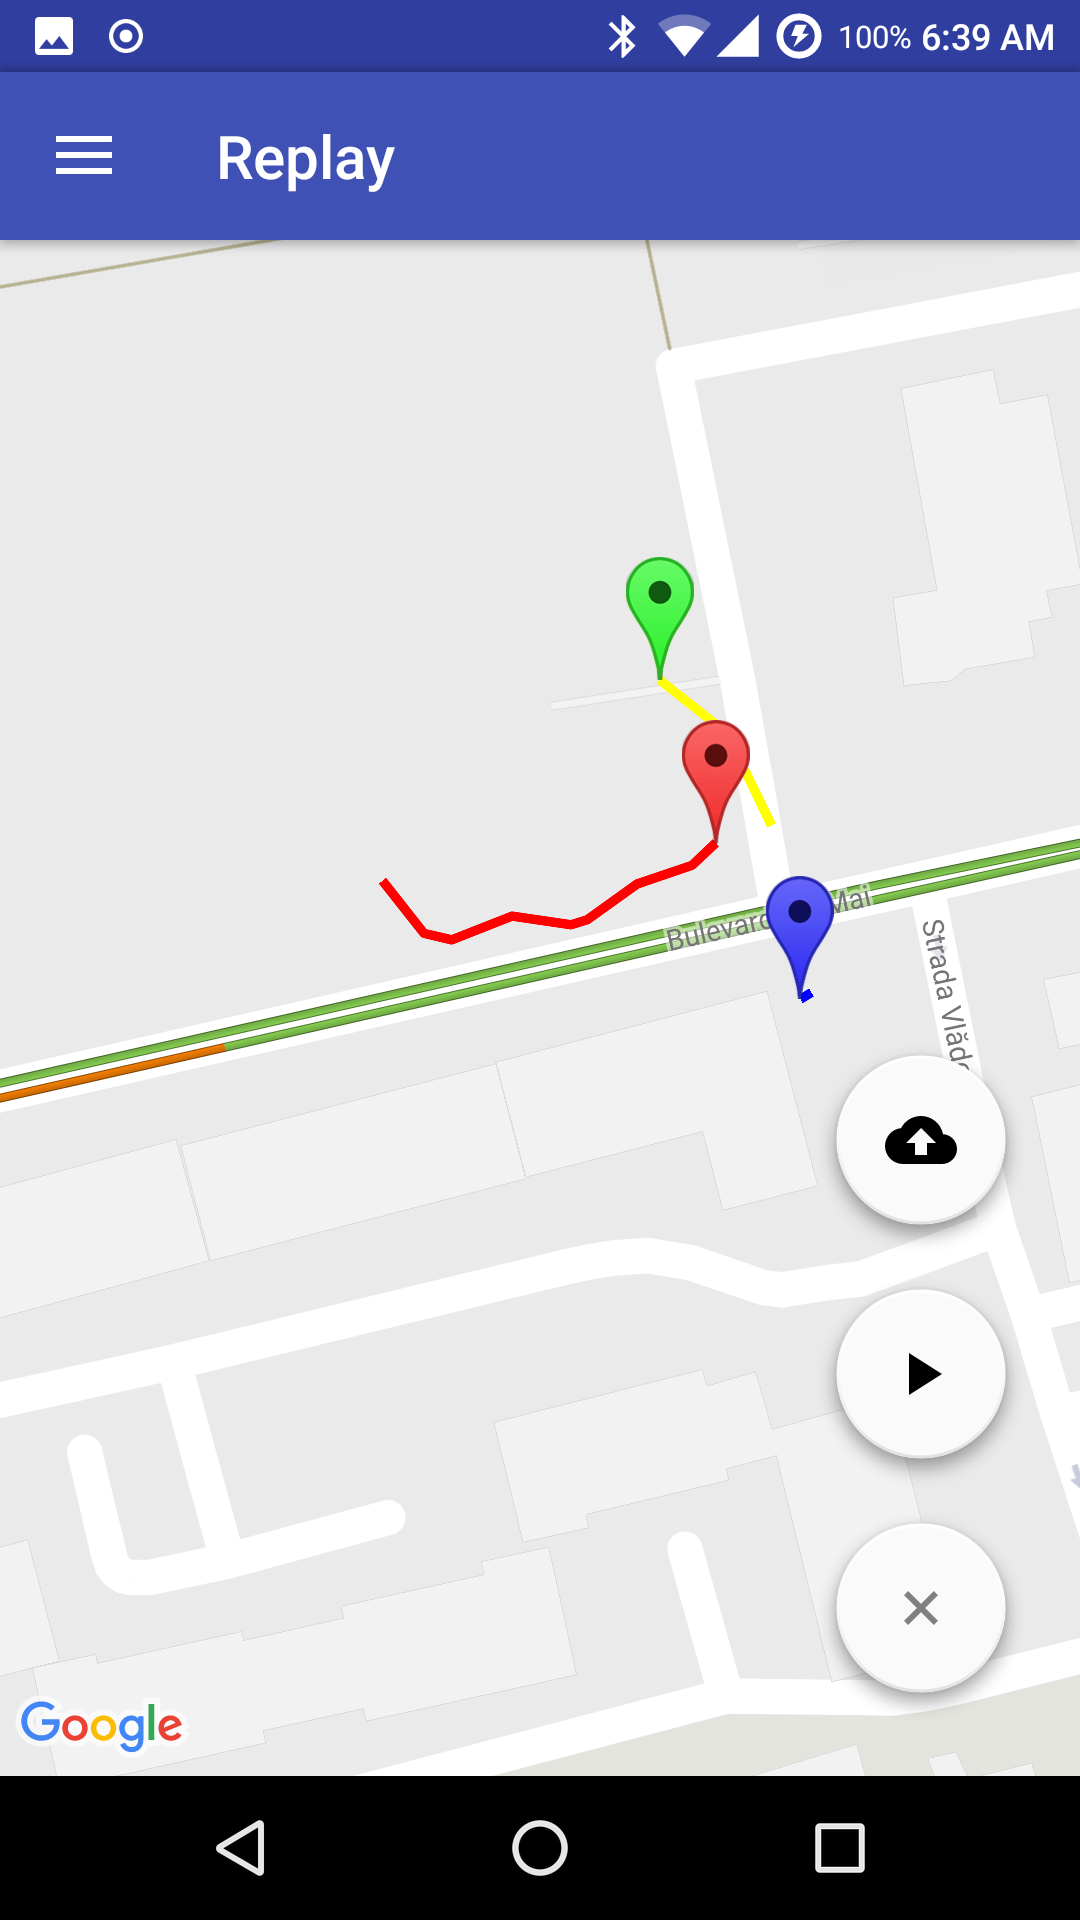
\includegraphics[scale=0.1]{replayfound}
\caption{\label{fig:replayfround}Replay Activity with Safe place found}
\end{wrapfigure}


\section{Conclusions and Future Work}
\label{sec:conclusions}
% vim: set tw=78 sts=2 sw=2 ts=8 aw et ai:

While the central server approach has the advantage of being easy to manage,
it also poses certain drawbacks. It is easy to imagine a scenario where
cellular connections of clients would drop because of overburdening a
single base station, or even the server.
Several criteria, such as Closeness to Friends, were not actually implemented,
but in fact the preference to each Safe Location was given equally as 1/n (n
being the total number of Safe Locations).


\bibliographystyle{abbrv}
\bibliography{paper}

\end{document}
